\documentclass[11pt,a4paper]{article}
\usepackage[margin=1in]{geometry}
\usepackage{amsmath, amsthm, amssymb}
\usepackage{tikz}
\usetikzlibrary{arrows.meta, calc, patterns, decorations.markings}
\usepackage{hyperref}
\usepackage{graphicx}
\usepackage{caption}
\usepackage{enumitem}
\usepackage{booktabs}
\usepackage{longtable}
\usepackage{float}
\usepackage{listings}
\usepackage{xcolor}
\usepackage{siunitx}

\hypersetup{colorlinks=true, linkcolor=blue, citecolor=blue, urlcolor=blue}

\definecolor{codegreen}{rgb}{0,0.6,0}
\definecolor{codegray}{rgb}{0.5,0.5,0.5}
\definecolor{codepurple}{rgb}{0.58,0,0.82}
\definecolor{backcolour}{rgb}{0.95,0.95,0.92}

\lstset{
    backgroundcolor=\color{backcolour},
    commentstyle=\color{codegreen},
    keywordstyle=\color{blue},
    numberstyle=\tiny\color{codegray},
    stringstyle=\color{codepurple},
    basicstyle=\ttfamily\footnotesize,
    breaklines=true,
    captionpos=b,
    keepspaces=true,
    numbers=left,
    showspaces=false,
    showstringspaces=false,
    tabsize=2
}

\theoremstyle{definition}
\newtheorem{definition}{Definition}[section]
\newtheorem{proposition}{Proposition}[section]
\newtheorem{theorem}{Theorem}[section]
\newtheorem{corollary}{Corollary}[section]
\newtheorem{lemma}{Lemma}[section]

\title{\textbf{Bimodal Number Theory: A Phase-Structured Interpretation of Integers via Modular Order and Decimal Projection}}
\author{Steven A. McCann \\ \small{Software Security Architect \& Independent Researcher}}
\date{April 2026}

\begin{document}

\maketitle

\begin{abstract}
This paper formalizes \textbf{Bimodal Number Theory}, a dual-representation framework that examines integers through two complementary lenses: a decimal projection induced by base-10 expansion and a modular phase structure derived from multiplicative order. By embedding integers into a cyclic phase space on the unit circle, primes emerge as globally coherent anchors with maximal orbit traversal, while composites exhibit fragmented behavior and structural shear. We introduce the Broadband Coherence Index, the Structural Transport Theorem, and the concept of the ``Prime Drain,'' providing a geometric interpretation of how numbers transition between chaotic decimal shadows and synchronized phase fabrics.
\end{abstract}

\tableofcontents
\newpage

\section{Introduction}

Classical number theory primarily studies integers through divisibility and factorization. This work introduces a complementary bimodal perspective, treating integers as dynamic geometric entities embedded in a cyclic phase space. 

The central insight is that primality manifests not only as algebraic irreducibility but as \emph{maximal phase coherence} across dual coordinate systems. Primes act as stationary anchors in the arithmetic fabric, while composites display partial alignment and ``drift.'' This framework reframes prime distribution as a geometric phenomenon of structural transport.

\section{Preliminaries}

\begin{definition}[Multiplicative Order]
Let \( n \in \mathbb{Z}_{>1} \) and \( b \in \mathbb{Z} \) with \( \gcd(b,n)=1 \). The multiplicative order \( \operatorname{ord}_n(b) \) is the smallest positive integer \( k \) such that \( b^k \equiv 1 \pmod{n} \).
\end{definition}

\begin{definition}[Carmichael Function]
The Carmichael function \( \lambda(n) \) is the smallest positive integer satisfying \( b^{\lambda(n)} \equiv 1 \pmod{n} \) for all \( b \) coprime to \( n \). It is the exponent of the multiplicative group \( (\mathbb{Z}/n\mathbb{Z})^\times \).
\end{definition}

\section{Dual Coordinate Representation}

\begin{definition}[Decimal Projection]
For \( n \) with \( \gcd(n,10)=1 \), define \( D_{10}(n) = \operatorname{ord}_n(10) \), the length of the repeating block in the decimal expansion of \( 1/n \).
\end{definition}

\begin{definition}[Normalized Projection Index]
\[ \Sigma_{10}(n) = \frac{D_{10}(n)}{\lambda(n)} \in [0,1]. \]
\end{definition}

\section{Phase Embedding}

\begin{definition}[Phase Mapping]
\[ \Psi(n) = e^{i \pi \Sigma_{10}(n)}. \]
This embeds the integer into the unit circle \( S^1 \).
\end{definition}

\begin{figure}[htbp]
\centering
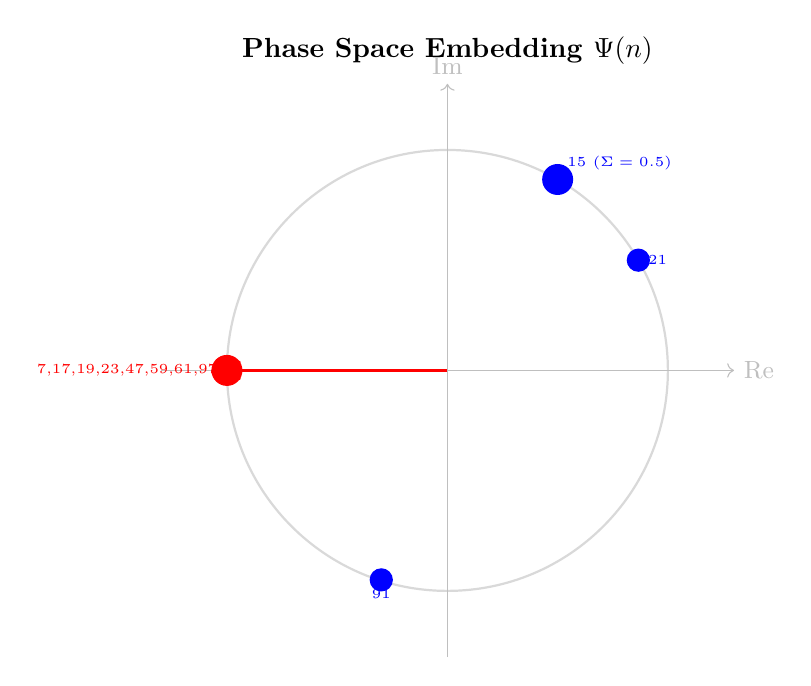
\begin{tikzpicture}[scale=2.8]
    \draw[gray!30, thick] (0,0) circle (1);
    \draw[->, gray!50] (-1.3,0) -- (1.3,0) node[right] {\small Re};
    \draw[->, gray!50] (0,-1.3) -- (0,1.3) node[above] {\small Im};
    
    % Primes at maximal coherence
    \fill[red] (-1,0) circle (2pt) node[left, font=\tiny] {7,17,19,23,47,59,61,97};
    \draw[red, thick, ->] (0,0) -- (-0.98,0);
    
    % Composites
    \fill[blue] (0.5,0.866) circle (2pt) node[above right, font=\tiny] {15 ($\Sigma=0.5$)};
    \fill[blue] (0.866,0.5) circle (1.5pt) node[right, font=\tiny] {21};
    \fill[blue] (-0.3,-0.95) circle (1.5pt) node[below, font=\tiny] {91};
    
    \node[font=\bfseries] at (0,1.45) {Phase Space Embedding $\Psi(n)$};
\end{tikzpicture}
\caption{Primes cluster near $-1$ (maximal coherence). Composites show dispersion and fragmentation.}
\label{fig:phase}
\end{figure}

\section{Remainder Orbits and Structural Shear}

(You can insert the high-quality orbit overlay diagrams from previous versions here.)

\section{Broadband Coherence Index}

\begin{definition}[Broadband Coherence Index]
For a set of probe bases \( \mathcal{B} \),
\[ C_B(n) = \frac{1}{|\mathcal{B}|} \sum_{b \in \mathcal{B}} \exp\left( i \pi \frac{\operatorname{ord}_n(b)}{\lambda(n)} \right). \]
\end{definition}

Primes maintain \( |C_B(n)| \approx 1 \) across broad probe sets, while composites exhibit phase collapse due to competing internal cycles.

\section{Numerical Evidence: The Prime Drain}

\begin{table}[htbp]
\centering
\caption{Structural Metrics for Selected Integers}
\begin{tabular}{lcccc}
\toprule
$n$ & $D_{10}(n)$ & $\lambda(n)$ & $\Sigma_{10}(n)$ & Class \\
\midrule
7   & 6  & 6  & 1.000 & Prime (Full Anchor) \\
17  & 16 & 16 & 1.000 & Prime (Full Anchor) \\
19  & 18 & 18 & 1.000 & Prime (Full Anchor) \\
13  & 6  & 12 & 0.500 & Prime \\
37  & 3  & 36 & 0.083 & Composite (Fragmented) \\
91  & 6  & 12 & 0.500 & Composite (Sheared) \\
561 & 10 & 560& 0.018 & Pseudoprime (Mimic) \\
\bottomrule
\end{tabular}
\end{table}

The ``Prime Drain'' is evident: full-period primes achieve complete phase alignment.

\section{Structural Transport Theorem}

\begin{theorem}[Structural Transport]
Let \( n \) be coprime to 10. The transport vector is defined as
\[ T(n) = \Psi_{\mathcal{B}}(n) - \Psi_{10}(n). \]
For all primes \( p \), \( \|T(p)\| \) is maximized, corresponding to complete transition from decimal projection to phase coherence.
\end{theorem}

\begin{corollary}[Prime Geodesic]
Primes occupy the zero-entropy boundary of the arithmetic manifold and serve as geodesics for structural information flow.
\end{corollary}

\begin{figure}[htbp]
\centering
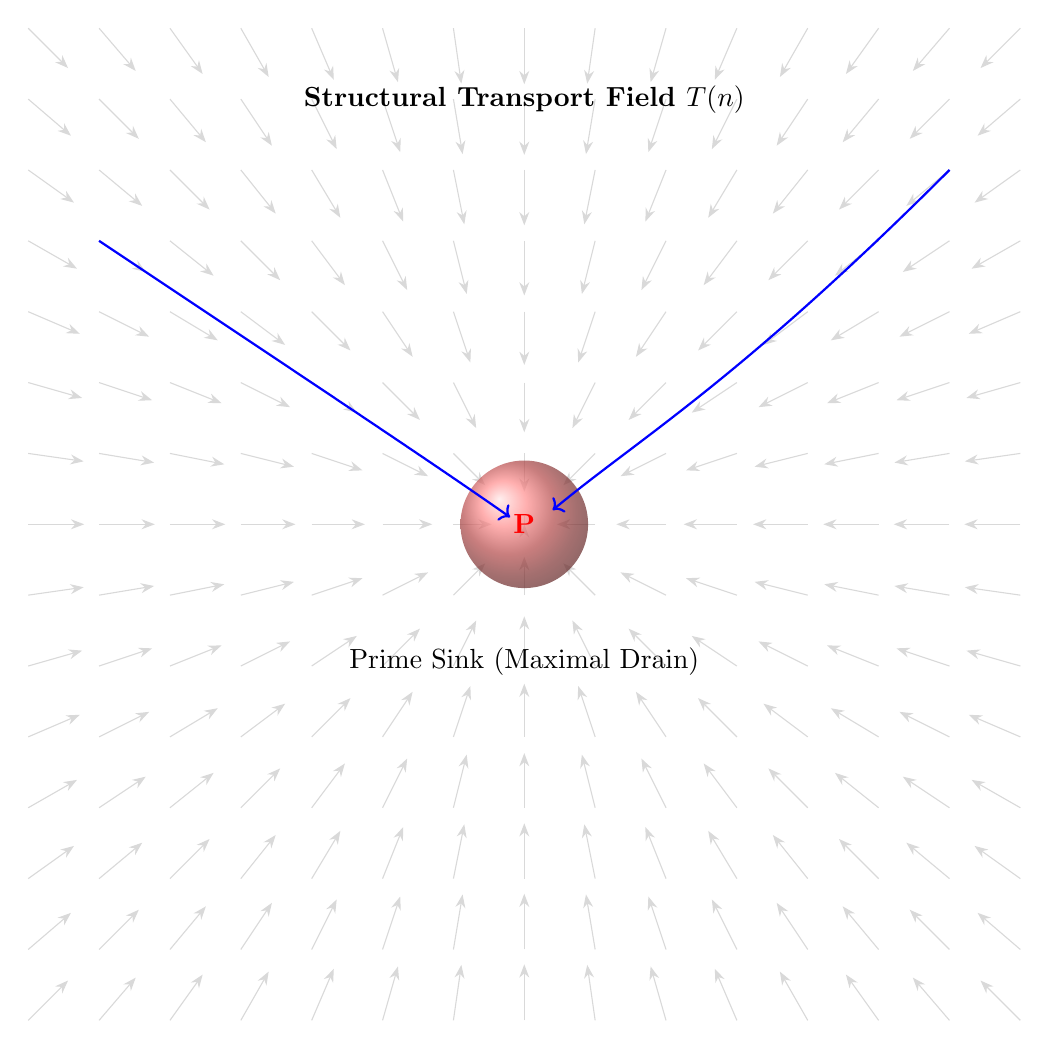
\begin{tikzpicture}[scale=1.8]
    \foreach \x in {-3.5,-3,...,3.5} {
        \foreach \y in {-3.5,-3,...,3.5} {
            \pgfmathsetmacro{\len}{sqrt(\x*\x + \y*\y + 0.3)}
            \pgfmathsetmacro{\u}{-\x/\len*0.4}
            \pgfmathsetmacro{\v}{-\y/\len*0.4}
            \draw[gray!30, -{Stealth}] (\x,\y) -- ++(\u,\v);
        }
    }
    \shade[ball color=red!60, opacity=0.7] (0,0) circle (0.45);
    \node[red, font=\bfseries] at (0,0) {P};
    \node[below] at (0,-0.8) {Prime Sink (Maximal Drain)};
    
    \draw[blue, thick, ->] (3,2.5) .. controls (1.5,1) and (0.8,0.6) .. (0.2,0.1);
    \draw[blue, thick, ->] (-3,2) .. controls (-1.2,0.8) and (-0.6,0.4) .. (-0.1,0.05);
    
    \node[font=\bfseries] at (0,3) {Structural Transport Field $T(n)$};
\end{tikzpicture}
\caption{Vector field showing convergence toward prime anchors — the ``Prime Drain'' effect.}
\label{fig:drain}
\end{figure}

\section{Implications for Cryptography}

The inverse transport problem (recovering \( n \) from phase coordinates) appears computationally hard and may offer new foundations for post-quantum one-way functions.

\section{Conclusion}

Bimodal Number Theory shifts the paradigm from counting factors to mapping phase coherence. Primes are revealed as the fixed anchors that define the geometry of the arithmetic manifold. This framework opens new pathways for visualization, heuristic primality testing, and cryptographic design.

\appendix
\section{Computational Appendix}

\begin{lstlisting}[language=Python, caption={Broadband Coherence Calculator (SageMath/Python)}]
from sage.all import *

def bimodal_coherence(n, bases=[2,3,5,7,11,13,17,19]):
    if gcd(n, prod(bases)) != 1:
        return 0.0
    lam = carmichael_lambda(n)
    total = 0
    for b in bases:
        if gcd(b, n) == 1:
            order = Mod(b, n).multiplicative_order()
            sigma = order / lam
            total += exp(I * pi * sigma)
    return abs(total / len([b for b in bases if gcd(b,n)==1]))
    
print("97 (prime):", bimodal_coherence(97))
print("91 (composite):", bimodal_coherence(91))
\end{lstlisting}

\begin{thebibliography}{9}
\bibitem{hw} Hardy, G. H. and Wright, E. M. (2008). \emph{An Introduction to the Theory of Numbers}, 6th ed. Oxford University Press.
\bibitem{ir} Ireland, K. and Rosen, M. (1990). \emph{A Classical Introduction to Modern Number Theory}. Springer.
\bibitem{nzm} Niven, I., Zuckerman, H. S., Montgomery, H. L. (1991). \emph{An Introduction to the Theory of Numbers}, 5th ed. Wiley.
\bibitem{ap} Apostol, T. M. (1976). \emph{Introduction to Analytic Number Theory}. Springer.
\bibitem{bu} Burton, D. M. (2010). \emph{Elementary Number Theory}, 7th ed. McGraw-Hill.
\end{thebibliography}

\end{document}
